\usetikzlibrary{arrows.meta,calc}
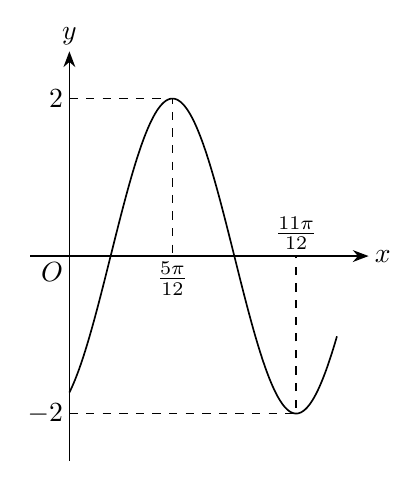
\begin{tikzpicture}[x=1cm,y=1cm,line width=.6pt,>=Stealth,font=\normalsize]
\draw[->] (-0.5,0)--(3.8,0) node[right,inner sep=0pt,xshift=2pt] {$x$};
\draw[->] (0,-2.6)--(0,2.6) node[above,inner sep=0pt,yshift=2pt] {$y$};
\node[below left,inner sep=0pt,xshift=-2pt,yshift=-2pt] at (0,0) {$O$};
\draw[dashed] (0,2)--(1.308,2)--(1.308,0);
\draw[dashed] (0,-2)--(2.88,-2)--(2.88,0);
\node[left,inner sep=0pt,xshift=-2pt] at (0,2) {$2$};
\node[left,inner sep=0pt,xshift=-2pt] at (0,-2) {$-2$};
\node[below,inner sep=0pt,yshift=-2pt] at (1.308,0) {$\frac{5\pi}{12}$};
\node[above,inner sep=0pt,yshift=2pt] at (2.88,0) {$\frac{11\pi}{12}$};
\draw[domain=0:3.4,samples=200] plot (\x,{2*sin(deg(2*\x)-60)});
\end{tikzpicture}
